\section{The Emergence of Heterogeneous Computing}

    For several decades, from the 1970s until the early 2000s, advances in
    processor development followed Moore's Law \citep{4785860} and
    Dennard Scaling \citep{1050511}.
    This meant that the density of integrated circuits approximately doubled
    every two years, and processor clock frequencies increased proportionally
    while maintaining steady power consumption.
    This enabled continual processor improvements that were driven primarily by
    rising clock frequencies and microarchitectural refinements, enabling ever
    faster computations.

    The physics-driven nature \citep{Hutcheson2018Moore} of these advances in
    hardware has had important implications for software development.
    Not only did the performance of computers improve exponentially, but these
    performance gains were in the form of direct speedups, available to all the
    already existing programs.
    The primary interfaces between software and hardware - the instruction set
    architectures of processors - evolved gradually and with few
    paradigmatic changes \citep{8310168}.
    This is best exemplified by the pervasive x86 instruction set architecture,
    which still retains backward compatibility with its original inception in
    1978, and dominates desktop processors to this day.
    Software developers and users could, therefore, rely on ever-increasing
    performance from hardware progress alone, without any intervention.

\subsection{Via Multi-Processing to Heterogeneous Compute}

    This continual progress started breaking down around 2005 with the apparent
    end of Dennard Scaling \citep{6307773}.
    While the shrinking of transistors continued, this no longer enabled
    proportionally increased clock frequencies with the same power budget.
    Processor designers instead started using the increasing transistor
    budget for adding additional processor cores.
    This shift toward multi-processing has left a deep mark on software
    development.
    New programming paradigms and languages, annotation systems, programming
    interfaces, libraries and compiler techniques were developed, and continue
    to evolve, to address the challenges of parallel computing.

    In recent years, transistor scaling has slowed significantly.
    In response to the now prevailing breakdown of both Dennard Scaling and
    Moore's Law, the hardware industry has turned toward architectural
    innovation \citep{7878935}.
    In particular, there is a trend toward specialised processor cores with
    that work in tandem as a heterogeneous system.
    Specialised processor cores outperform general-purpose cores on specific
    tasks.
    Furthermore, as heat dissipation has become a major challenge,
    simultaneously powering all transistors is often unviable, meaning that
    different processor cores have to be masked out dynamically at runtime
    (``dark silicon'') \citep{6307773}.
    Disabling a subset of a homogeneous multi-core system renders some of its
    cores redundant, whereas specialised cores can improve the system
    performance overall even if they are disabled most of the time and only
    used for the specific tasks at which they excel.

\section{The Diminished Role of Traditional Compilers}

    Heterogeneous computing can help overcome the scaling limitations of
    homogeneous, general-purpose processors.
    However, it also poses an enormous challenge to the associated software
    ecosystem, and it puts into question many of the achievements in portability
    and longevity of programs that are taken for granted in modern computing
    \citep{8719512}.
    Existing software does not automatically benefit from entirely new
    accelerator designs in the way that it profited from continuous
    improvements of established architectures.
    Where previously, programs performed better on each succeeding hardware
    generation, with at most a recompilation required, new accelerators arrive
    with novel and incompatible interfaces.

    In particular, this new hardware landscape greatly diminishes the scope of
    responsibilities and impact that traditional compilers for languages such as
    C, C++ and Fortran can have.
    Such compilers used to be responsible for orchestrating
    program execution on the entirety of available computing resources.
    They are now generally limited to only targeting the relatively small
    homogeneous fraction of processor cores directly.

\subsection{Libraries and Domain-Specific Languages Fill the Gap}

    In order to reach peak performance on rapidly evolving and highly parallel
    hardware, novel programming models built around libraries and
    domain-specific languages have emerged.
    They succeed in utilising heterogeneous hardware in situations where
    traditional compilers fail.

    Two examples display the diversity of these approaches:
    Firstly, \citet{Ragan-Kelley2013Halide} developed the domain-specific
    language Halide for image processing.
    The Halide toolchain is able to generate fast code for heterogeneous
    platforms by focusing on a well-understood class of computations and by
    using a restrictive program representation.
    After tuning programs for particular platforms, it outperforms
    hand-optimised code, demonstrating an immense potential for domain-specific
    compiler optimisation under circumstances of constrained semantics.

    Secondly, Basic Linear Algebra Subprograms (BLAS)
    \citep{2002:USB:567806.567807}, a standard for library function interfaces
    going back to \citet{Lawson:1979:BLA:355841.355847} in the 1970s, have been
    implemented for most accelerators.
    These implementations are widely used and offer unrivalled performance.
    Some versions are provided directly by hardware vendors to support
    accelerators \citep{mkl,cublas,clblas,apl,qml}, while others originate as
    academic projects \citep{Wang:2013:AAG:2503210.2503219}.
    These different competing implementations use a plethora of approaches to achieve as
    close to peak performance as possible.
    This includes manually written assembly code, but also highly advanced
    code generation techniques, custom program representations and many more.

\subsection{Negative Consequences of Declining Compiler Scope}

    Domain-specific languages and library interface make the full performance of
    heterogeneous systems accessible to programs.
    These success stories, however, leave significant problems unaddressed.
    The adoption costs are high, requiring application rewrites for
    accelerators.
    This coincides with often uncertain long-term prospects and minimal
    cross-platform portability.
    Even in the case of the agreed-upon BLAS standard -- arguably the best case
    scenario -- adoption of novel implementations is non-trivial in practice,
    due to the frequently encountered interface extensions for managing device
    handlers and memory synchronisation.
    For academic-backed domain-specific languages like Halide, on the other
    hand, complete rewrites are required in entirely novel ecosystems, with an
    entirely unclear future of support.

    On heterogeneous systems, programmers relied on compilers for mainstream
    programming languages to evolve alongside processor development.
    Even decades-old C++ source code can be compiled into efficient programs for
    the newest generation x86 processors.
    The pervasive requirement for domain specific-languages and libraries only
    arises because compilers are unable to map programs to specialised cores.
    Compilers are therefore increasingly downgraded to merely coordinating the
    launch of core workloads in the form of computational kernels, which are
    then executed as separate and opaque programs.
    In order to improve this situation, it is important to consider from a
    distance the reasons for these compiler shortcomings.

    It may appear obvious that e.g.\ a full C++ or Java compiler cannot be
    provided for a typical graphics processor -- after all, most graphics
    processors have hardware limitations that prevent them from implementing the
    entire language standard.
    Indeed, many accelerators are even further from Turing complete.
    However, this should not prevent a partial compiler, offloading suitable
    subprograms, while falling back on homogeneous hardware providing a full
    language implementation for the remainder.
    After all, that is exactly the result achieved with libraries and
    domain-specific languages as well, and likely the desirable outcome.
    Despite the obvious convenience of such an approach, the next section shows
    that there are important reasons why this has not been championed so far.

\section{Host Compilers and Kernel Compilers}
    
    An important first observation is that a specific class of compilers already
    plays an important role in targeting heterogeneous hardware.
    Many of the kernel programs that remain opaque to the application compilers
    are themselves products of other, specialised compilers.
    This necessitates a distinction between {\em host compilers} and {\em kernel
    compilers}.
    This distinction is mirrored of course by the differences between {\em host
    languages} and {\em kernel languages}.
    The two classes of compilers have developed quite distinctly.
    Kernel compilers successfully apply many of the techniques that have had
    only limited success for host compilers.
    They reason automatically about parallelism, understand data dependencies at
    a deeper level, and they incorporate iterative compilation.

    This is made possible by a combination of factors that apply uniquely to
    kernel compilers.
    Smaller programs allow for more expensive compilation techniques;
    more restrictive languages and intermediate representations allow for
    stronger reasoning;
    abstractions in kernel compilers can be customised for the exact hardware
    architecture of accelerators;
    and domain knowledge from areas such as image processing can be directly
    embedded in custom compiler technology, without requiring their validity
    on generic programs.
    Furthermore, kernel compilers often run in more controlled environments,
    with less need for predictability, reproducibility and stability.
    The range of input programs might even be small enough to leave compilation
    to experts and vendors, which may share the results in the form of already
    compiled library functions.

    As host compilers operate under less forgiving conditions, it is
    unsurprising that they have lagged behind these developments.
    Because they cannot rely on such a restricted environment, host compilers
    are unable to match the optimisation capabilities of kernel compilers.
    Domain specific compilers and languages, as well as libraries, have
    therefore not been championed only because their restricted program
    spaces match the capabilities of particular heterogeneous accelerators.
    The restricted environment also makes them intrinsically more powerful and
    able to generate better code.

    Hybrid approaches, such as OpenCL, reinforce these observations.
    The language is domain specific only in its expression of parallelism, but
    otherwise designed to be general purpose.
    Compilers are provided for many structurally different processors.
    However, as a consequence of being a relatively unrestricted language, the
    compilers often underperform and the language is notoriously lacking in
    performance portability.
    Partial compilers that require the same kinds of compromises as OpenCL --
    unable to utilize the restricted nature of input programs -- would suffer
    the same shortcomings.

\subsection{The Spectrum of Specialisation}

    General purpose programming languages, domain specific languages and
    accelerator libraries exist on a spectrum of specialisation.
    \Cref{specialgradient} gives some intuition about this spectrum.
    On the left are the most versatile general purpose languages.
    Moving to the right, flexibility is lost, with BLAS libraries at the end
    providing only fixed-function computations.
    At the same time however, the restricted semantics allow for greater 
    optimisation capabilities.

    It is important to clarify here what is meant by optimisation potential in
    this context and how it differs from raw performance.
    C++ is of course very suitable for manual optimisation.
    However, it is difficult for compilers to automatically perform deep
    structural changes to the program.
    Maintaining the semantics of BLAS routines, on the other hand, is viable
    with many structurally different implementation approaches.
    C++ is fast because of its low overhead and because programmers write
    efficient programs to begin with, BLAS is fast because the semantics are so
    constrained that implementations can be tuned to perfection.

\begin{figure}[t]
\centering
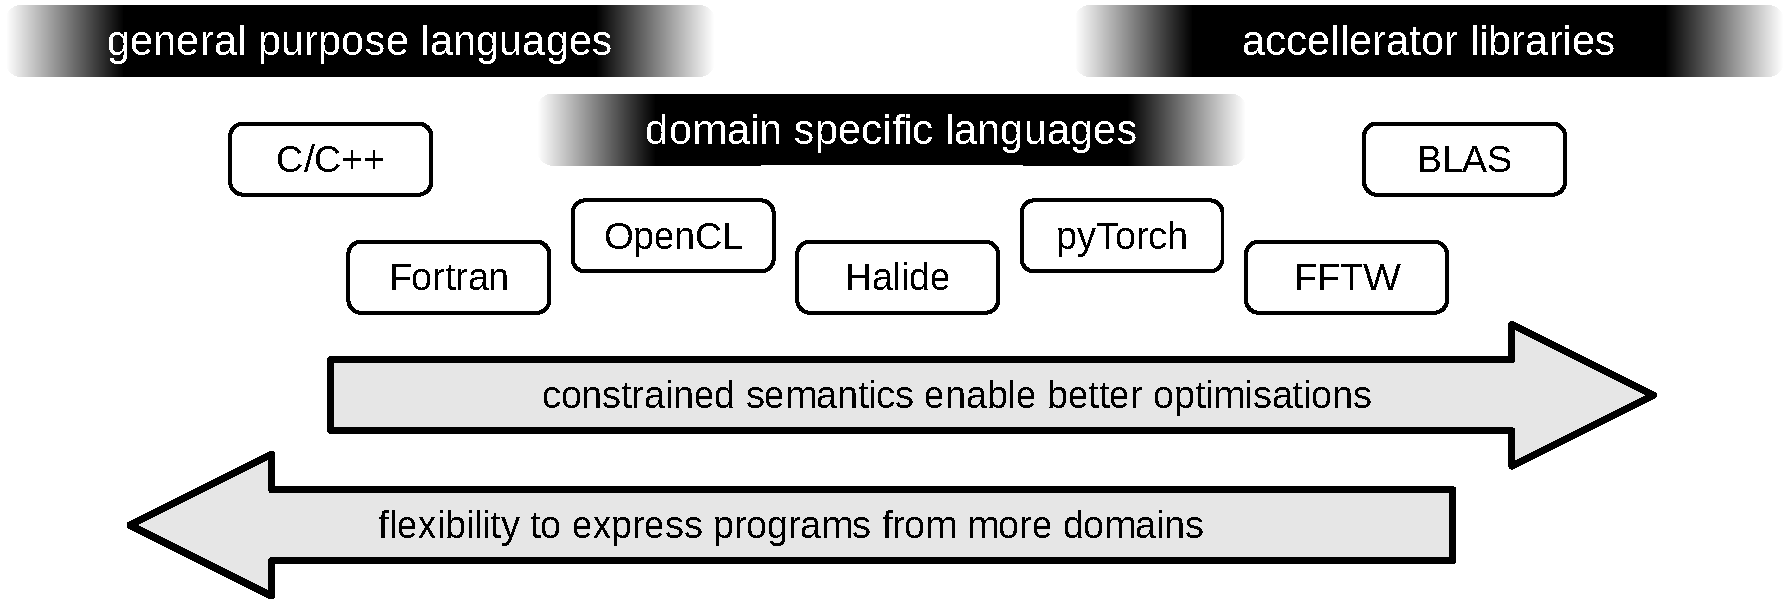
\includegraphics[width=\textwidth]{figures/DSLgradient}
\caption{Domain specific languages on a spectrum between general purpose
         languages and libraries.
         Decreasing flexibility allows for stronger reasoning and greater
         optimisation potential.}
\label{specialgradient}
\end{figure}

    The additional performance that libraries and domain specific kernel
    compilers achieve on suitable applications is a consequence of operating
    under more constrained conditions.
    While expert programmers can often apply this domain knowledge themselves
    when using general purpose languages, this potential is automatically
    uncovered with specialised tools.
    The restrictions imply domain knowledge that are leveraged to make stronger
    assumptions, use more powerful models and generate better code.

    {\bf
    When compilers operate on more constrained models, they have more
    optimisation opportunities and they achieve higher performance and better
    portability.
    The models that compilers use are mostly a reflection of the input
    programming language.
    However, if host compiler could recognise program parts that adhere
    to a stronger model with more restrictions, their disadvantage against
    kernel compilers and libraries should vanish.
    }

\section{Moving Between Abstraction Levels}

    To combine the positive features on both ends of the spectrum in
    \Cref{specialgradient}, host compilers need the ability to recognise
    restricted programming models within general purpose code and to transform
    adhering code sections into domain specific representations.
    After these transformations, host compilers would be able to tap into the
    extensive knowhow that already exists by utilising specialised code
    generation techniques.

    Conceptually, this approach has been applied in specific domains before.
    Some polyhedral compilers take as input arbitrary code, but they recognise
    whether parts of code are actually expressible in the much more restricted
    polyhedral model.
    If possible, they reformulate the code into this system and continue
    optimisation with domain knowledge, thus resulting in better code.
    This thesis will develop a broad generalization of this concept, extending
    far beyond polyhedral code regions and encompassing a methodology that
    needs no commitment to one specific model.

\subsection{Program Specialization with Constraints}

    Program code typically passes through a whole range of representations
    during compilation with a modern, general purpose compiler.
    Starting from the textual source code, an abstract syntax tree is built,
    from which a serialised intermediate representation is constructed,
    which is then passed on to the compiler back end for code generation.
    The intermediate representation -- typically in static single assignment
    form -- is used for the majority of optimising code transformations.
    This best represents the semantic model, and therefore the set of
    assumptions and capabilities, that the compiler uses to represent the
    program.

    Static single assignment form representations are accessible to mathematical
    reasoning, with most of their interesting properties based on graph and list
    structures.
    With this in mind, structural restrictions on intermediate representation
    code -- corresponding to restricted, domain specific models -- can be
    precisely formulated as mathematical constraints.
    Established methods around constraint solvers then make an automatic
    detection of adhering code regions feasible.

    This constraint programming methodology needs to capture the spectrum from
    \Cref{specialgradient}.
    On one extreme, sections of code should be recognised as implementing
    specific algorithms, like matrix multiplications, that are merely
    parametrised with numbers.
    Next are algorithms that allow parametrisation with an operator.
    Stencil kernels or reductions fall into this category.
    More generic again are programs that merely follow specific structural
    restrictions.
    Polyhedral code sections fall under this domain.

\section{Conclusion}

    This thesis develops a framework to formulate a wide range of restricted
    program models using constraints.
    For this purpose, a custom constraint programming language is introduced
    and successively extended.
    Starting from theoretical foundations, the methodology is developed into
    a complete system, implemented as part of the mature Clang C/C++ compiler.

    In the later chapters, this core system is then applied in combination
    with other techniques in a range of different contexts.
    This includes the rapid prototyping of compiler optimisations, the
    automatic parallelisation of program structures with indirect memory
    accesses, a new formulation of the polyhedral model and the detection of
    computational structures that cover important bottlenecks in typical
    scientific programs.
    
    Eventually, the techniques are combined with memory synchronisation
    approaches to result in a fully integrated, extensible compiler tool for
    efficiently mapping sequential programs onto heterogeneous systems.
    This develops the thesis all the way from theoretical discussions of
    constraint programming approaches in compilers to the evaluation of real
    performance improvements on established benchmark suites and scientific
    applications.

%    \subsection*{extra building blocks}



%    The thesis develops a methodology to generalize this approach, resulting in
%    methods by which compilers can automatically classify code as adhering to
%    additional semantic constraints beyond what is guaranteed by the programming
%    language.
%    Using this classification, the compiler can then translate the code into a
%    more specialized domain and apply the already developed domain specific
%    techniques -- in the simplest case by merely linking to a library -- to
%    achieve full performance.


%    The implication of this is that in order to achieve best performance, it is
%    generally advisable to choose the most specialised tools available.
%    However, considerations of portability and maintainability push programmers
%    in the opposite direction, towards a small number of well established host
%    compilers and traditional languages at the expense of performance.



%    What is promising therefore is a combination of hand-optimised libraries,
%    domain specific languages together with compiler automatisms.
%    This requires a disruptive improvement in compiler analysis capabilites.
%    The detection of higher level algorithmic structures in compilers has been
%    investigated before, but established approaches cannot scale to what
%    this challenge requires.
%    Syntactic matching directly on programming languages has become
%    unviable for the complexities of both modern programming languages and
%    complex code bases.

%    Instead, this thesis develops an entirely novel approach based on concepts
%    from constraint solving, building a pragmatic methodology for detecting
%    complex algorithmic structures -- computational idioms.

%    In order to successfully target heterogeneous systems, host compilers need
%    to leverage the know-how that already exists in the surrounding software
%    ecosystem, encapsulated in special purpose libraries and code generators.

%    A linear alebra compiler operates under the assumption that the program is
%    linear algbera, and the program representation that is used with not even
%    allow the expression of any other system.

\newpage
\section{Structure of the Thesis}

    This thesis is divided into six chapters.
    Following this introduction, the core methodology is developed in
    {\bf\Cref{chapter:theory}}.
    This forms the basis of the later
    {\bf\Cref{chapter:candl,chapter:idioms,chapter:reductions}}.
    Based on a novel mathematical model of established static single assignment
    form compiler representations, a constraint programming approach is derived
    and some particular challenges are discussed in detail.

    {\bf\Cref{chapter:literature}} gives a broad overview of the related work.
    This literature survey covers the four main research areas that this work
    is placed in.
    Firstly {\em constraint programming}, which is the basis of the methodology
    for most of this research.
    Secondly {\em compiler analysis and auto-parallelisation}, against which the
    results in this thesis are evaluated.
    Thirdly {\em heterogeneous computing}, which motivates many of the compiler
    approaches that this research enables.
    Lastly {\em computational idioms}, a term for several overlapping concepts
    of algorithmic patterns.

    {\bf\Cref{chapter:candl,chapter:idioms,chapter:reductions}}
    are each based on a published research article and elaborate on different
    applications of constraint programming in compilers.

    {\bf\Cref{chapter:candl}} develops a full-fledged constraint programming
    language called CAnDL, with an implementation in the LLVM compiler
    infrastructure that automatically generates compiler analysis passes from
    declarative descriptions.
    Using CAnDL, the chapter explores several complex compiler analysis
    challenges, concluding with a full polyhedral code analysis.
    The work of this chapter has been published as
    {\bf\citet{Ginsbach:2018:CDS:3178372.3179515}}.

    {\bf\Cref{chapter:reductions}} develops an auto-parallelising compiler for
    complex reduction and histogram computations using CAnDL-powered analysis
    functionality.
    This covers many computations that are inaccessible to established
    approaches based on data flow or polyhedral analysis and is to demonstrate
    the greater flexibility of constraint programming.
    The work of this chapter has been published as
    {\bf\citet{ginsbach2017discovery}}.

    {\bf\Cref{chapter:idioms}} extends CAnDL into the Idiom Description Language
    (IDL) and applies it to algorithmic concepts that go beyond traditional
    compiler analysis: stencil computations, complex reductions and histograms
    as well as sparse and dense linear algebra.
    The resulting automatic detection passes in LLVM enable automatic
    heterogeneous acceleration of sequential code and result in significant
    speedups on established benchmark suites.
    The work of this chapter has been published as
    {\bf\citet{Ginsbach:2018:AML:3173162.3173182}}.
